\chapter{Conclusions}

\section{Summary}

A measurement of the production of a {\PW} and a $\PZ$ boson in association with two jets has been presented,
using events where both bosons decay leptonically.
Results are based on data corresponding to an integrated luminosity of $35.9\fbinv$
recorded in proton-proton collisions at $\sqrt{s} = 13\TeV$ with the CMS detector
at the LHC in 2016. The cross section in a tight fiducial region with enhanced contributions from
electroweak (EW) \WZ production is $\sigma^{\mathrm{fid}}_{\WZjj} = 3.18^{+0.71}_{-0.63}\unit{fb}$,
consistent with the standard model (SM) prediction.
The dijet mass and dijet rapidity separation are used to measure
the signal strength of \EWWZ production with
respect to the SM expectation, resulting in
$\mu_{\EW} = 0.82^{+0.51}_{-0.43}$.
The significance of this result is
2.2 standard deviations with 2.5 standard deviations expected.
at $13\TeV$.
This is the first study of this process performed by the CMS Collaboration.

Constraints are placed on anomalous quartic gauge couplings
in terms of dimension-eight effective field theory operators, and
upper limits are given on the production cross section
times branching fraction of charged Higgs bosons.
The upper limits on charged Higgs boson production
via vector boson fusion with decay to a {\PW} and a {\cPZ} boson
extend the results previously published
by the CMS Collaboration~\cite{Sirunyan:2017sbn} and
are comparable to those of the ATLAS Collaboration~\cite{Aaboud:2018ohp}.
These are the first limits for dimension-eight effective field theory
operators in the \WZ channel at $13\TeV$.

\section{Outline}

The \WZjj and \EWWZ cross section measurements are statistically limited.
Therefore, a significant reduction in the uncertainty is expected from
analyzing a larger data set. The CMS experiment collected data from
13\TeV LHC collisions in 2017 and 2018, corresponding to data sets
of 41.1 and 59.7\fbinv of integrated luminosity.
By combining the results obtained here with
an analysis performed on this data set, sensitivity to the \EWWZ process
within sensitivity exceeding 5 standard is expected with only moderate
reductions in the systematic uncertainties. Increase statistics will
also allow differential measurements of the \WZjj process to be made.
A measurement with a 50\% reduction in the uncertainty would be sensitive
to the large corrections NLO \EW corrections observed for the $\Wpm\Wpm$
VBS process and demonstrated in preliminary studies for \WZjj.


\begin{figure}[htbp]
  \centering
   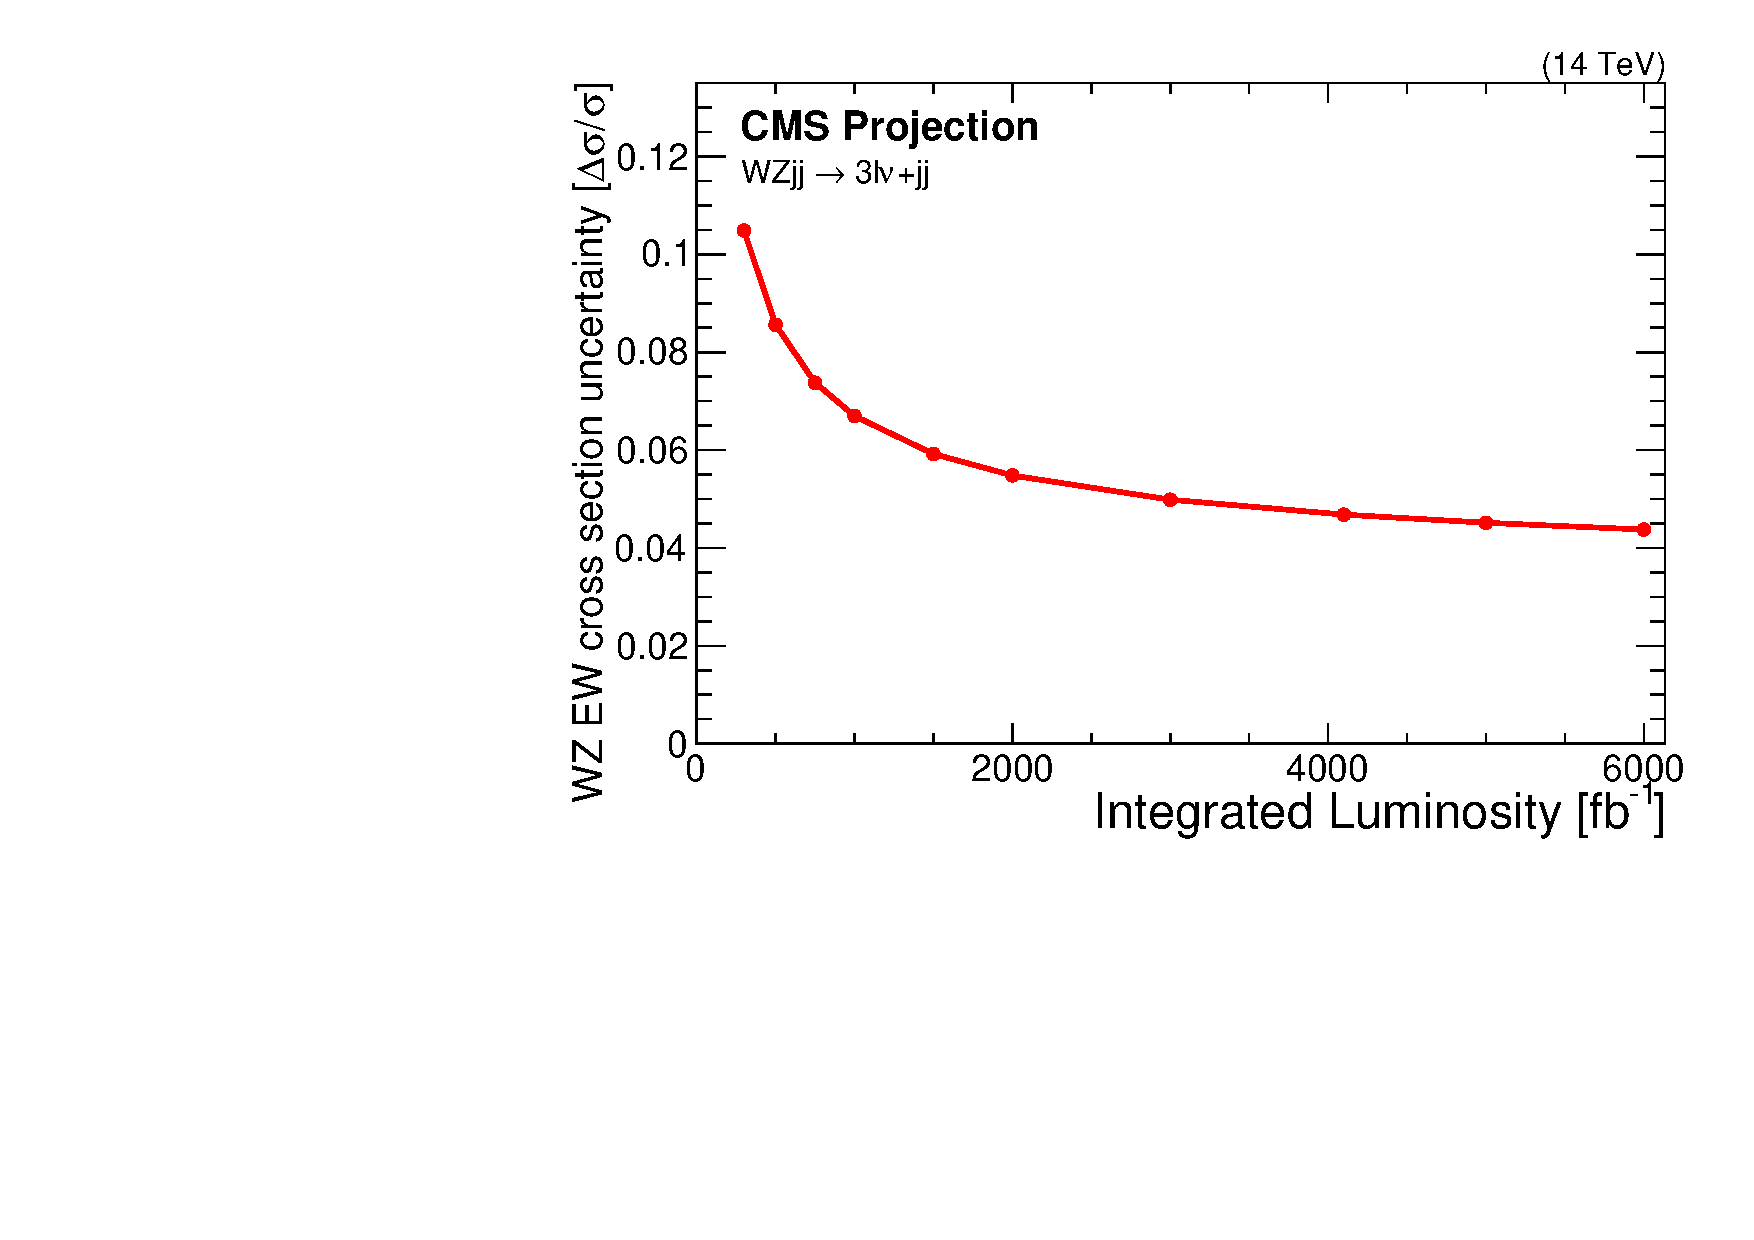
\includegraphics[width=0.6\textwidth]{figures/Conclusions/WZjjSignficanceHLLHC.pdf}
  \caption{
    Reproduced from Ref.~\cite{CMS-PAS-FTR-18-038}.
        }
 \label{fig:WZHLLHC}
\end{figure}
